We now return to the case study outlined in section \ref{sec:casestudy}. We analyze two scenarios. In figure \ref{fig:experiment}, we have 6 available mobile sensors. We compare the surveillance strategy with the situation in figure \ref{fig:3experiment} where we have only 6. Our surveillance task is $\LTLsquare \LTLdiamond p_5$, i.e, we need to infinitely often bring the belief of the target location to 5 cells or lower. 

\begin{figure}
\subfloat[The gridworld in \ref{fig:SGR-grid} partitioned into 6 subgames. \label{fig:experiment}]{
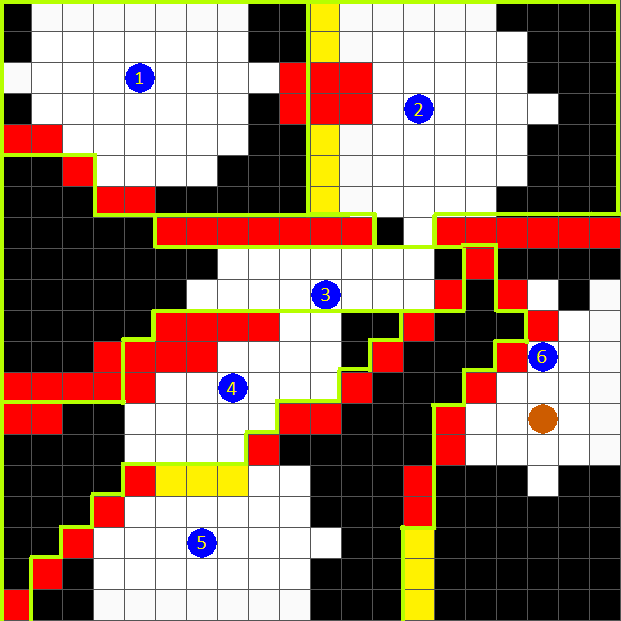
\includegraphics[scale=0.18]{figs/SGR-grid-vis-part.png}
\hspace{.3cm}}
%\hfill
\subfloat[The gridworld in \ref{fig:SGR-grid} partitioned into 3 subgames. \label{fig:3experiment}]{
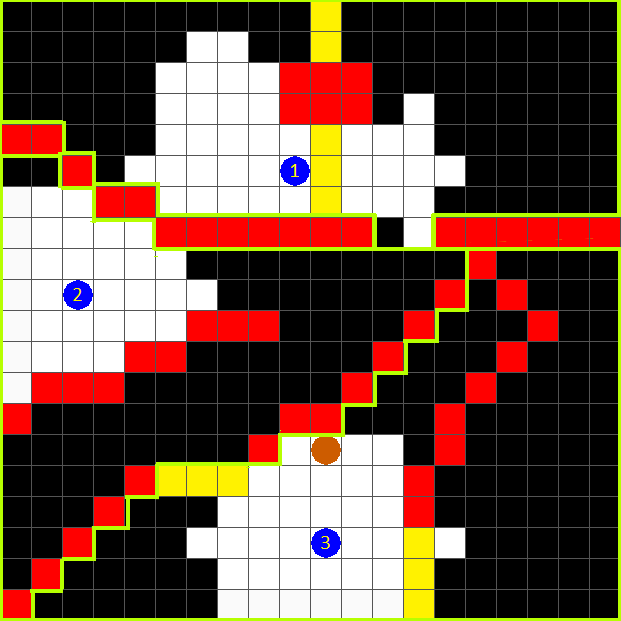
\includegraphics[scale=0.18]{figs/SGR-grid-vis-part_3.png}
\hspace{.3cm}}

\caption{We look at the case where we have 6 mobile sensors in \ref{fig:experiment} and 3 mobile sensors \ref{fig:3experiment}\label{fig:bigexp}}. The mobile sensors or UAVs are blue circles and the target is represented in orange. The red cells represent impassable terrain (such as dense foliage) that cannot be seen through by the sensors. Black cells are locations not visible to any sensor.
\end{figure} 

Solving either case centralized is not computationally feasible as the state space grows exponentially with the number of sensors. We partition the multi-agent surveillance game into subgames as shown in Figures \ref{fig:experiment} and \ref{fig:3experiment}. We then solve each game individually in report the synthesis times in table \ref{tab:synthtime}.

\begin{table}[h!]
	\centering
	\caption{Synthesis times for surveillance games}
	\label{tab:synthtime}
	\begin{tabular}{c|l|l}
		\multicolumn{1}{l|}{}                                    & \textbf{Subgame} & \textbf{Synthesis time (s)} \\ \hline \hline
		\multirow{7}{*}{\textbf{6 sensors}}                     & Subgame 1        & 40                          \\
		& Subgame 2        & 38                          \\
		& Subgame 3        & 49                          \\
		& Subgame 4        & 44                          \\
		& Subgame 5        & 33                          \\
		& Subgame 6        & 39                          \\ \hline
		& \textbf{Total}            & 245                         \\ \hline
		\multicolumn{1}{l|}{\multirow{4}{*}{\textbf{3 sensors}}} & Subgame 1        & 187                         \\
		\multicolumn{1}{l|}{}                                    & Subgame 2        & 251                         \\
		\multicolumn{1}{l|}{}                                    & Subgame 3        & 211                         \\
		\multicolumn{1}{l|}{}                                    & \textbf{Total}            & 684                        
	\end{tabular}
\end{table}

The multi-agent surveillance game in figure \ref{fig:experiment} results in more sub-games compared to the game in \ref{fig:experiment}. However, each game is much smaller and results in a much faster synthesis time individually. 